\documentclass[12pt]{article}
\usepackage[top=1in,left=1in, right = 1in, footskip=1in]{geometry}

\usepackage{graphicx}
%\usepackage{adjustbox}

\newcommand{\eref}[1]{(\ref{eq:#1})}
\newcommand{\fref}[1]{Fig.~\ref{fig:#1}}
\newcommand{\Fref}[1]{Fig.~\ref{fig:#1}}
\newcommand{\sref}[1]{Sec.~\ref{#1}}
\newcommand{\frange}[2]{Fig.~\ref{fig:#1}--\ref{fig:#2}}
\newcommand{\tref}[1]{Table~\ref{tab:#1}}
\newcommand{\tlab}[1]{\label{tab:#1}}
\newcommand{\seminar}{SE\mbox{$^m$}I\mbox{$^n$}R}

\usepackage{amsthm}
\usepackage{amsmath}
\usepackage{amssymb}
\usepackage{amsfonts}

%\usepackage{lineno}
%\linenumbers

\usepackage[pdfencoding=auto, psdextra]{hyperref}

\usepackage{natbib}
\bibliographystyle{chicago}
\date{\today}

\usepackage{xspace}
\newcommand*{\ie}{i.e.\@\xspace}

\usepackage{color}

\newcommand{\Rx}[1]{\ensuremath{{\mathcal R}_{#1}}} 
\newcommand{\Ro}{\Rx{0}}
\newcommand{\RR}{\ensuremath{{\mathcal R}}}
\newcommand{\Rhat}{\ensuremath{{\hat\RR}}}
\newcommand{\tsub}[2]{#1_{{\textrm{\tiny #2}}}}

\newcommand{\comment}[3]{\textcolor{#1}{\textbf{[#2: }\textsl{#3}\textbf{]}}}

%% \newcommand{\rev}[1]{\comment{red}{REV}{#1}}
\newcommand{\rev}[1]{}

\newcommand{\swp}[1]{\comment{magenta}{SWP}{#1}}
\newcommand{\new}[1]{\textcolor{blue}{#1}}

\begin{document}

\begin{flushleft}{
	\Large
	\textbf\newline{
		Assessing uncertainties associated with early estimates of the basic reproduction number during the novel coronavirus (2019-nCoV) outbreak
	}
}
\newline
\\
Sang Woo Park\textsuperscript{1}
Jonathan Dushoff\textsuperscript{2,3}
\\

\bigskip
\textbf{1} Department of Ecology and Evolutionary Biology, Princeton University, Princeton, New Jersey, USA
\\
\textbf{2} Department of Biology, McMaster University, Hamilton, Ontario, Canada
\\
\textbf{3} Michael G. DeGroote Institute for Infectious Disease Research, McMaster University, Hamilton, Ontario, Canada
\\
\bigskip

% *swp2@princeton.edu
\end{flushleft}

\section*{Abstract}

\pagebreak

As the novel coronavirus (2019-nCoV) continues to spread,
researchers are rushing to publish their estimates of the basic 
reproductive number $\mathcal R_0$.
The basic reproductive number (i.e., the 
average number of secondary cases generated 
by a primary case in a fully susceptible population) is of particular interest 
because it allows prediction about the final size of an epidemic.
While their efforts are valuable, their analyses rely on several
assumptions that could immediately affect their estimates of $\mathcal R_0$ and
the associated uncertainties in their estimates.
Here, we illustrate the degree to which their assumptions can affect
their estimates and stress few principles that needs to be taken into
consideration.

\section*{Early estimates of $\mathcal R_0$}

Early in an outbreak, $\mathcal R_0$ cannot be estimated directly,
whereas the exponential growth rate $r$ can be estimated reliably.
Given estimates of the exponential growth rate $r$ and the distribution $g(\tau)$ of 
generation intervals (i.e., the time between when a person become 
infected and that person infects another person), the basic reproduction
number can be estimated via the Euler-Lotka equation:
\begin{equation}
1/\mathcal R_0 = \int \exp(-r\tau) g(\tau) d\tau.
\end{equation}
Therefore, early estimates of $\mathcal R_0$ must 
necessarily depend on the assumptions about $r$ and $g(\tau)$.


\begin{figure}[t]
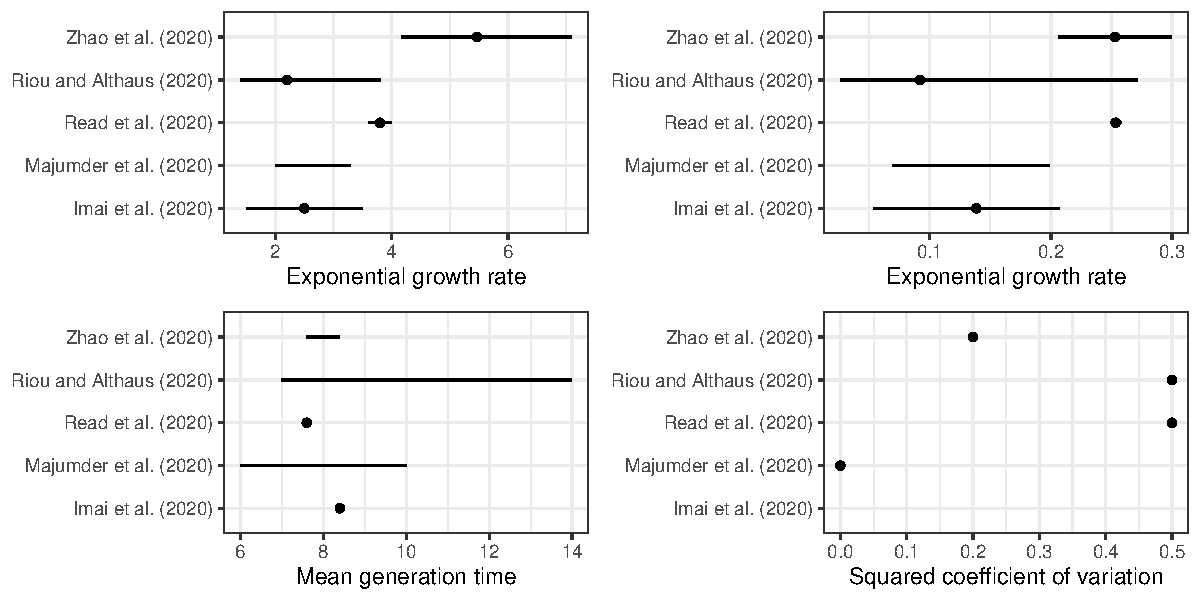
\includegraphics[width=\textwidth]{../fig/comparison.pdf}
\caption{
Early estimates of $\mathcal R_0$ and associated assumptions about $r$ and $g(\tau)$.
}
\end{figure}

We use the gamma approximation framework to demonstrate
how assumptions about $r$ and $g(\tau)$
affects $\mathcal R_0$.
Assuming that generation intervals follow a gamma distribution 
with the mean $\bar G$ and the squared coefficient of variation $\kappa$, 
we have
\begin{equation}
\mathcal R_0 = \left(1 + \kappa r \bar{G}\right)^{1/\kappa}.
\end{equation}
This equation demonstrates that generation-interval distributions
with a larger mean (higher $\bar{G}$) or less variability (lower $\kappa$)
will give a higher estimate of $\mathcal R_0$.
Likewise, strong assumptions about $\bar{G}$ and $\kappa$ will give
estimates of $\mathcal R_0$ with narrow confidence intervals.

Figure 1 clearly demonstrates the lack of uncertainties in the underlying parameters
of the current $\mathcal R_0$ estimates.
In particular, no studies properly propagate uncertainties associated with the
amount of variability in generation intervals, which can have 
large effects on the estimates of $\mathcal R_0$
For example, when the relative mean generation interval is long ($r\bar{G}\approx 2$ based on the estimates by \cite{zhaoncov}),
varying $\kappa$ from 0 to 1 reduces the estimate of $\mathcal R_0$ by more than a two fold.

To assess the amount of uncertainties in the estimate of $\mathcal R_0$,
we come up with distributions that span over the assumptions made by other people:
\begin{equation}
\begin{aligned}
r &\sim \mathrm{Gamma}(\alpha=5, \beta=5/0.15)\\
\bar{G} &\sim \mathrm{Gamma}(\alpha=10, \beta=10/8.5)\\
\kappa &\sim \mathrm{Gamma}(\alpha=10, \beta=10/0.35)\\
\end{aligned}
\end{equation}
These give median estimate of $\mathcal R_0$ of 2.37 with 95\% qunatile of 1.26--9.01.

\begin{table}[!th]
\begin{center}
\begin{tabular}{l|c|c|c|c}
Study & $\mathcal R_0$ & $r$ ($\textrm{days}^{-1}$) & $\bar G$ (days) & $\kappa$ \\
\hline
\cite{imaincov} & 2.5 (1.5--3.5) & 0.14 (0.05--0.21) & 8.4 & unspecified$^\ast$ \\
\hline
\cite{majumderncov} & 2.0--3.3 & 0.07--0.20 & 6--10 & 0 \\
\hline
\cite{readncov} & 3.8 (3.6--4.0) & 0.25 (0.25--0.26)$^\dagger$ & 7.6 & 0.5 \\
\hline
\cite{riouncov} & 2.2 (1.4--3.8) & 0.09 (0.03--0.27) & 7--14 & 0.5\\
\hline
\cite{zhaoncov} & 5.47 (4.16--7.1)$^\ddagger$ & 0.25 (0.21--0.30) & 7.6--8.4 & 0.2
\end{tabular}
\end{center}
\caption{
\textbf{Parameter estimates and assumptions}
Exponential growth rate $r$ is calculated by using the following formula: $r = (\mathcal R_0^\kappa - 1)/(\kappa \bar{G})$.
$^\ast$We assume $\kappa = 0.5$ to calculate $r$.
$^\dagger$Exponential growth rate $r$ is calculated by using the exact formula for the SEIR model \citep{ma2014estimating}.
$^\ddagger$Assuming no increase in the reporting rate.
}
\end{table}




\bibliography{wuhan}

\end{document}
